Pour créer un réseau \ac{P2P} entre navigateurs, Netflux utilise la technologie \acf{WebRTC}.
\ac{WebRTC} est une API\footnote{\ac{API} : Interface de Programmation} de navigateur spécifiée en 2011, et en cours d'implémentation dans les différents navigateurs depuis 2013.
Elle permet de créer une connexion directe entre deux navigateurs pour échanger des médias audio et/ou vidéo, ou simplement des données.

Cette API utilise pour cela un ensemble de protocoles.
Ces protocoles réintroduisent des serveurs dans l'architecture système de MUTE.
Dans la \autoref{fig:architecture-systeme-webrtc}, nous représentons une collaboration réalisée avec \ac{MUTE}, composé de noeuds formant un réseau \ac{P2P}, de différents serveurs nécessaires à la mise en place du réseau \ac{P2P}.
Finalement, nous représentons les interactions entre les noeuds et ces serveurs.

\begin{figure}[!ht]
  \centering
  \includegraphics[page=3, trim=7cm 3cm 4cm 2cm, clip, width=.7\linewidth]{img/mute-figures.pdf}
  \caption{Architecture système pour la couche réseau de MUTE}
  \label{fig:architecture-systeme-webrtc}
\end{figure}

Nous décrivons ci-dessous le rôle respectif de chaque type de serveur dans la collaboration.
